% =====================================================================
\chapter{Relaciones de equivalencia y de orden}
\label{tema:5}
% =====================================================================

Una relación binaria expresa que dos elementos están «relacionados» de cierta manera: ser iguales módulo~$n$, tener la misma longitud, preceder a otro. Este tema estudia las dos familias de relaciones más importantes, las de equivalencia, que clasifican, y las de orden, que ordenan. Sigue el capítulo~11 de Hammack~\cite{hammack}, las secciones~4.2 a~4.5 de Velleman~\cite{velleman} y las secciones~4.4 y~9.6 a~9.10 de~\cite{mcs}.

\section{Relaciones binarias}

\begin{definicion}[Relación]
Una \emph{relación} (binaria) en un conjunto $A$ es un subconjunto $R\subseteq A\times A$. Se escribe $a\,R\,b$ si $(a,b)\in R$.
\end{definicion}

\begin{ejemplo}
En $\Z$: la igualdad, el orden $\le$, la divisibilidad $a\mid b$ (existe $k\in\Z$ con $b=ka$) y la congruencia módulo $n$, $a\equiv b\pmod n$ si $n\mid(a-b)$. En $\Sigma^{*}$: «tener la misma longitud» y «ser prefijo de». Toda función $f\colon A\to B$ es una relación entre $A$ y $B$ (\cref{def:t2-funcion}).
\end{ejemplo}

Una relación en un conjunto finito puede representarse con un grafo dirigido, con un arco $a\to b$ por cada par $(a,b)\in R$, o con una matriz de ceros y unos cuya entrada $(a,b)$ vale~1 si $a\,R\,b$.

\begin{definicion}[Propiedades]\label{def:t5-prop}
Una relación $R$ en $A$ es
\begin{enumerate}
  \item \emph{reflexiva} si $a\,R\,a$ para todo $a\in A$;
  \item \emph{simétrica} si $a\,R\,b$ implica $b\,R\,a$;
  \item \emph{antisimétrica} si $a\,R\,b$ y $b\,R\,a$ implican $a=b$;
  \item \emph{transitiva} si $a\,R\,b$ y $b\,R\,c$ implican $a\,R\,c$.
\end{enumerate}
\end{definicion}

\begin{center}\small
\begin{tabular}{@{}lcccc@{}}
\toprule
Relación & Reflexiva & Simétrica & Antisimétrica & Transitiva \\
\midrule
$=$ en $\Z$ & sí & sí & sí & sí \\
$\le$ en $\Z$ & sí & no & sí & sí \\
$<$ en $\Z$ & no & no & sí & sí \\
$\mid$ en $\N$ & sí & no & sí & sí \\
$\equiv$ (mód.\ $n$) en $\Z$ & sí & sí & no & sí \\
$\neq$ en $\Z$ & no & sí & no & no \\
\bottomrule
\end{tabular}
\end{center}

Simetría y antisimetría \emph{no} son contrarias: la igualdad tiene ambas, y la relación $\{(1,2),(2,1),(1,3)\}$ en $\{1,2,3\}$ no tiene ninguna.

\section{Relaciones de equivalencia y particiones}

\begin{definicion}[Relación de equivalencia]
Una relación $\sim$ en $A$ es de \emph{equivalencia} si es reflexiva, simétrica y transitiva. La \emph{clase de equivalencia} de $a\in A$ es $[a]=\{x\in A: x\sim a\}$, y el \emph{conjunto cociente} es $A/{\sim}=\{[a]: a\in A\}$.
\end{definicion}

\begin{definicion}[Partición]
Una \emph{partición} de $A$ es una familia de subconjuntos de $A$ no vacíos, disjuntos dos a dos y cuya unión es $A$.
\end{definicion}

\begin{teorema}\label{teo:t5-particion}
Sea $\sim$ una relación de equivalencia en $A$. Entonces:
\begin{enumerate}
  \item $a\in[a]$ para todo $a$;
  \item $[a]=[b]$ si y solo si $a\sim b$;
  \item dos clases son iguales o disjuntas.
\end{enumerate}
En consecuencia, $A/{\sim}$ es una partición de $A$. Recíprocamente, toda partición $\mathcal{C}$ de $A$ define una relación de equivalencia, $a\sim b$ si $a$ y $b$ están en el mismo bloque de $\mathcal{C}$, cuyas clases son los bloques.
\end{teorema}

\begin{proof}
(i) Por la reflexividad. (ii) Si $[a]=[b]$, entonces $a\in[a]=[b]$, es decir, $a\sim b$. Recíprocamente, sea $a\sim b$; si $x\in[a]$, entonces $x\sim a$ y $a\sim b$, luego $x\sim b$ por transitividad, y $x\in[b]$; así $[a]\subseteq[b]$. Por simetría $b\sim a$, y el mismo argumento da $[b]\subseteq[a]$. (iii) Si $x\in[a]\cap[b]$, entonces $x\sim a$ y $x\sim b$; por simetría y transitividad, $a\sim b$, y por~(ii), $[a]=[b]$.

Por (i), las clases son no vacías y cubren $A$; por (iii), son disjuntas dos a dos: forman una partición. Para el recíproco, la relación «estar en el mismo bloque» es reflexiva porque los bloques cubren $A$, simétrica de forma evidente y transitiva porque, si $a,b$ comparten bloque y $b,c$ también, los dos bloques contienen a $b$ y son el mismo por ser disjuntos los distintos.
\end{proof}

\begin{ejemplo}[Enteros módulo $n$]\label{ej:t5-modn}
La congruencia módulo~3 tiene tres clases: $[0]=\{\dots,-3,0,3,6,\dots\}$, $[1]=\{\dots,-2,1,4,\dots\}$ y $[2]=\{\dots,-1,2,5,\dots\}$. El cociente se denota $\Z_3=\{[0],[1],[2]\}$~\cite[§11.5]{hammack}. Cada entero está en la clase de su resto al dividir entre~3.
\end{ejemplo}

\begin{proposicion}[Núcleo de una función]\label{prop:t5-nucleo}
Sea $f\colon A\to B$. La relación $a\sim_f a'$ si $f(a)=f(a')$ es de equivalencia, y sus clases son las fibras no vacías $f^{-1}(\{b\})$, $b\in f(A)$.
\end{proposicion}

La demostración es el \cref{eje:5-nucleo}. Muchas relaciones de equivalencia son de este tipo: «tener la misma longitud» es el núcleo de $\ell\colon\Sigma^{*}\to\N$, y la congruencia módulo $n$ es el núcleo de la función «resto de dividir entre $n$».

\section{Relaciones de orden}

\begin{definicion}[Orden]
Una relación $\preceq$ en $A$ es un \emph{orden parcial} si es reflexiva, antisimétrica y transitiva; el par $(A,\preceq)$ es un \emph{conjunto ordenado}. Es un \emph{orden total} si, además, dos elementos cualesquiera son comparables: $a\preceq b$ o $b\preceq a$. Un elemento $m$ es \emph{minimal} si no existe $x\neq m$ con $x\preceq m$, y \emph{mínimo} si $m\preceq x$ para todo $x$; análogamente se definen maximal y máximo.
\end{definicion}

\begin{ejemplo}\label{ej:t5-ordenes}
(1) $\le$ en $\R$ es un orden total. (2) La inclusión $\subseteq$ en $\Pa(A)$ es un orden parcial, no total si $\abs{A}\ge2$: $\{a\}$ y $\{b\}$ no son comparables. (3) La divisibilidad en $\N$ es un orden parcial; en $\Z$ no es antisimétrica, porque $2\mid-2$ y $-2\mid2$. (4) El \emph{orden lexicográfico} en $\N\times\N$, $(a,b)\preceq(c,d)$ si $a<c$, o $a=c$ y $b\le d$, es un orden total; es el orden de un diccionario.
\end{ejemplo}

Un conjunto ordenado finito se representa con su \emph{diagrama de Hasse}: se dibuja un segmento ascendente de $x$ a $y$ cuando $x\prec y$ y no hay ningún $z$ con $x\prec z\prec y$; la reflexividad y la transitividad quedan implícitas (\cref{fig:t5-hasse}).

\begin{figure}[h]
\centering
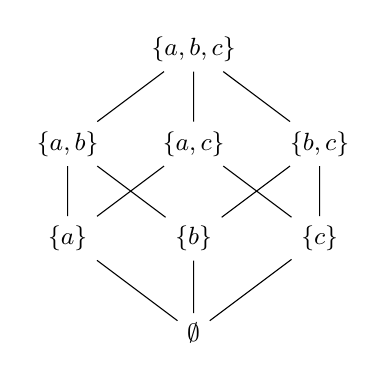
\begin{tikzpicture}[font=\small,node distance=1.1cm and 1.5cm]
  \node (e) at (0,0) {$\emptyset$};
  \node (a) at (-1.6,1.2) {$\{a\}$};
  \node (b) at (0,1.2) {$\{b\}$};
  \node (c) at (1.6,1.2) {$\{c\}$};
  \node (ab) at (-1.6,2.4) {$\{a,b\}$};
  \node (ac) at (0,2.4) {$\{a,c\}$};
  \node (bc) at (1.6,2.4) {$\{b,c\}$};
  \node (abc) at (0,3.6) {$\{a,b,c\}$};
  \draw (e)--(a) (e)--(b) (e)--(c) (a)--(ab) (a)--(ac) (b)--(ab) (b)--(bc) (c)--(ac) (c)--(bc) (ab)--(abc) (ac)--(abc) (bc)--(abc);
\end{tikzpicture}
\caption{Diagrama de Hasse de $(\Pa(\{a,b,c\}),\subseteq)$. El mínimo es $\emptyset$ y el máximo, $\{a,b,c\}$.}
\label{fig:t5-hasse}
\end{figure}

\begin{observacion}[Conexión con el curso]
Normalizar texto (pasar a minúsculas, aplicar una forma normal de Unicode) define el núcleo de una función y, por la \cref{prop:t5-nucleo}, una relación de equivalencia: dos cadenas son equivalentes si se normalizan igual (módulo~12, tema~1); la deduplicación de corpus agrupa documentos en clases de «casi duplicados» (módulo~16). Las relaciones de orden aparecen en el grafo computacional de una red, cuyo orden topológico es un orden total compatible con un orden parcial (módulo~10); en la atención causal, la posición $i$ solo atiende a las posiciones $j\le i$ (módulo~13); y BPE desempata entre pares igual de frecuentes con un orden total fijado (módulo~12, §2.3).
\end{observacion}

\begin{observacion}[Errores frecuentes]
(1) Creer que la simetría y la transitividad implican la reflexividad: el argumento «$a\sim b$ y $b\sim a$ dan $a\sim a$» exige que exista algún $b$ relacionado con $a$ (\cref{eje:5-error}). (2) Tratar simetría y antisimetría como contrarias. (3) Confundir elemento minimal con mínimo: en $\{2,3,4,6\}$ ordenado por divisibilidad, $2$ y $3$ son minimales y no hay mínimo. (4) Olvidar comprobar que una operación sobre clases no depende del representante elegido.
\end{observacion}

\begin{lecturas}
\item Hammack~\cite{hammack}, cap.~11 «Relations», §11.1–11.5.
\item Velleman~\cite{velleman}, §4.2 «Relations», §4.4 «Ordering Relations» y §4.5 «Equivalence Relations».
\item Lehman, Leighton y Meyer~\cite{mcs}, §4.4 «Binary Relations», §9.6 «Partial Orders», §9.8 «Linear Orders» y §9.10 «Equivalence Relations».
\end{lecturas}

\section*{Ejercicios del tema 5}
\addcontentsline{toc}{section}{Ejercicios del tema 5}

\begin{ejercicio}{1}{eje:5-propiedades}
En $A=\{1,2,3\}$ se consideran $R_1=\{(1,1),(2,2),(3,3),(1,2),(2,1)\}$, $R_2=\{(1,2),(2,3),(1,3)\}$, $R_3=\{(1,1),(2,2),(3,3)\}$ y $R_4=\{(1,2),(2,1)\}$. Decida para cada una si es reflexiva, simétrica, antisimétrica y transitiva.
\end{ejercicio}

\begin{ejercicio}{2}{eje:5-enteros}
Estudie las cuatro propiedades de la \cref{def:t5-prop} para las relaciones en $\Z$: (a) $a\,R\,b$ si $a+b$ es par; (b) $a\,R\,b$ si $ab\ge0$; (c) $a\,R\,b$ si $\abs{a-b}\le1$. ¿Cuál es de equivalencia? Describa sus clases.
\fuente{adaptado de Hammack~\cite{hammack}, §11.2 «Properties of Relations», ejercicios de la sección.}
\end{ejercicio}

\begin{ejercicio}{2}{eje:5-contar}
Sea $A$ un conjunto con $n=3$ elementos. ¿Cuántas relaciones hay en $A$? ¿Cuántas son reflexivas? ¿Cuántas simétricas? ¿Cuántas reflexivas y simétricas a la vez? Dé las fórmulas para $n$ general.
\end{ejercicio}

\begin{ejercicio}{2}{eje:5-clases}
Describa las clases de equivalencia y el conjunto cociente de: (a) la congruencia módulo~4 en $\Z$; (b) la relación en $\R^{2}$ «estar a la misma distancia del origen»; (c) la relación «tener la misma longitud» en $\{\cad{a},\cad{b}\}^{*}$, indicando cuántos elementos tiene cada clase.
\end{ejercicio}

\begin{ejercicio}{2}{eje:5-particion}
Sea $A=\{1,2,3,4,5,6\}$ y la partición $\{\{1,2\},\{3\},\{4,5,6\}\}$. Escriba los pares de la relación de equivalencia asociada y cuente cuántos son. Generalice: si los bloques tienen tamaños $k_1,\dots,k_r$, ¿cuántos pares tiene la relación?
\end{ejercicio}

\begin{ejercicio}{2}{eje:5-bell}
¿Cuántas relaciones de equivalencia hay en $\{1,2,3\}$? ¿Y en $\{1,2,3,4\}$? Clasifíquelas según los tamaños de los bloques de la partición correspondiente.
\end{ejercicio}

\begin{ejercicio}{3}{eje:5-modn}
Sea $n\ge1$. Demuestre que la congruencia módulo $n$ es una relación de equivalencia en $\Z$ y que tiene exactamente $n$ clases, $[0],[1],\dots,[n-1]$.
\fuente{adaptado de Hammack~\cite{hammack}, §11.3 «Equivalence Relations» y §11.5 «The Integers Modulo $n$».}
\end{ejercicio}

\begin{ejercicio}{3}{eje:5-nucleo}
Sea $f\colon A\to B$. Demuestre la \cref{prop:t5-nucleo}: la relación $a\sim_f a'$ si $f(a)=f(a')$ es de equivalencia y sus clases son las fibras no vacías de $f$. Deduzca que $f$ es inyectiva si y solo si todas sus clases tienen un solo elemento.
\fuente{adaptado de University of Washington, Math 300~\cite{uw300}, «Problems on functions», problema~3.}
\end{ejercicio}

\begin{ejercicio}{3}{eje:5-divide}
En $\N_{\ge1}=\{1,2,3,\dots\}$ se define $a\,R\,b$ si $a\mid b$ o $b\mid a$. ¿Es $R$ una relación de equivalencia? Demuestre las propiedades que se cumplan y refute las que no.
\fuente{adaptado de Cambridge, IA Numbers and Sets~\cite{camns}, Example Sheet~1, pregunta~10.}
\end{ejercicio}

\begin{ejercicio}{3}{eje:5-mas3}
Sea $R$ la relación en $\Z$ dada por $a\,R\,b$ si $b=a+3$. Se dice que una relación $S$ \emph{contiene} a $R$ si $a\,R\,b$ implica $a\,S\,b$. ¿Cuántas relaciones de equivalencia en $\Z$ contienen a $R$? Demuestre la respuesta.
\fuente{adaptado de Cambridge, IA Numbers and Sets~\cite{camns}, Example Sheet~1, pregunta~11.}
\end{ejercicio}

\begin{ejercicio}{3}{eje:5-fracciones}
En $X=\Z\times(\Z\setminus\{0\})$ se define $(a,b)\sim(c,d)$ si $ad=bc$. Demuestre que $\sim$ es una relación de equivalencia y describa la clase de $(1,2)$. Explique por qué $X/{\sim}$ puede identificarse con $\Q$.
\end{ejercicio}

\begin{ejercicio}{3}{eje:5-orden-partes}
(a) Demuestre que $\subseteq$ es un orden parcial en $\Pa(A)$, y que no es total si $\abs{A}\ge2$. (b) Demuestre que la divisibilidad es un orden parcial en $\N_{\ge1}$ y que no es antisimétrica en $\Z$.
\fuente{adaptado de Velleman~\cite{velleman}, §4.4 «Ordering Relations».}
\end{ejercicio}

\begin{ejercicio}{2}{eje:5-hasse}
(a) Dibuje el diagrama de Hasse de los divisores positivos de~12 ordenados por divisibilidad e indique minimales, maximales, mínimo y máximo. (b) Ordene lexicográficamente las cadenas $\cad{ab}$, $\cad{a}$, $\cad{b}$, $\cad{ba}$, $\cad{aab}$ y $\vacia$ (con $\cad{a}<\cad{b}$ y con la convención de que un prefijo propio precede a la cadena que lo contiene).
\end{ejercicio}

\begin{ejercicio}{3}{eje:5-lex}
Demuestre que el orden lexicográfico en $\N\times\N$ del \cref{ej:t5-ordenes} es un orden total. ¿Es un orden total el orden producto, $(a,b)\sqsubseteq(c,d)$ si $a\le c$ y $b\le d$?
\end{ejercicio}

\begin{ejercicio}{1}{eje:5-error}
Se afirma: «toda relación simétrica y transitiva es reflexiva, porque si $a\,R\,b$, la simetría da $b\,R\,a$ y la transitividad da $a\,R\,a$». Señale el error y dé un contraejemplo en $A=\{1,2\}$.
\end{ejercicio}
